\par \IEEEPARstart{F}{i}nalizada la enumeraci\'on de ciertos rubros que motiven la investigaci\'on sobre el tema, con la adici\'on de una breve perspectiva del problema a trabajar, nos centraremos a desarrollar con mayor precisi\'on, cada m\'etodo n\'umerico en cuesti\'on. Recordemos que estas herramientas encaminar\'an a las posible soluciones al problema de construir, a partir de un video en tiempo real, una secuencia de im\'agenes generadas de forma artificial que explaye la sensaci\'on de que el video original ha sido alentizado (efecto de $slowmotion$).

\subsection{Aclaraciones \'utiles para la comprensi\'on del desarrollo}

Antes de ingresar al campo que abarca la explicaci\'on de los m\'etodos, queremos esclarecer ciertas frases o palabras claves que ocupar\'an terreno en el resto de la secci\'on:

\begin{itemize}
	\item \textit{Frame original}: Se le dar\'a nombre al cuadro que pertenece al video original, es decir, aquel archivo que no contiene los frames agregados que conciben al efecto de c\'amara lenta.
	\item \textit{Frame artificial}: Lo llamaremos a aquellos cuadros que se realizar\'an a partir del procedimiento que dicho m\'etodo vaya planeando. En esta ocasi\'on, se puede ratificar que los mismos se crearan en conjunto, y entre medio de un par de frames originales.
	\item \textit{Cantidad de frames a adjuntar}: Nos referiremos al par\'ametro que decide cu\'antos cuadros artificiales le adicionaremos entre cada par de frames originales. Lo denotaremos con la letra $f$.
	\item \textit{Matriz frame}: Aunque no se hablar\'a de ese nombre en particular, es fundamental aclarar que en cualquier comentario acerca de los valores o p\'ixeles de un frame, se lo est\'a especificando como una matriz de $m$ x $n$ (visto como la resoluci\'on del video) que lleva los valores del $0$ al $255$, inclusive (escala de grises).
	\item \textit{P\'ixel}: Transladamos esta palabra asociada a la im\'agen digital al campo del \'algebra lineal. Por lo tanto, se lo considerar\'a como un componente de la matriz frame cuyos valores estan restringido en el rango $[0;255]$.
\end{itemize}

\subsection{Los m\'etodos propuestos}

\subsubsection{Cuadro m\'as cercano}

Este m\'etodo se basa en una idea de car\'acter simplista, pero comprende de una intuici\'on que puede resultar de utilidad para ciertos tipos de videos, como por ejemplo, la filmaci\'on de un objeto inm\'ovil.

Se extrae cada cuadro/frame en el orden en que el video los reproduce y tomando de a pares, se le adiciona una cierta cantidad de frames de por medio. No hay un n\'umero exacto que represente esta cantidad, por lo que se lo interpreta como par\'ametro de experimentaci\'on. Sin embargo, nos resta como inc\'ognita, el procedimiento por el cual se obtiene dichos cuadros. Esto \'ultimo es lo que caracterizar\'a al m\'etodo en cuesti\'on.

Nos abstraemos por un momento de la totalidad de frames que compone una grabaci\'on para analizar en detalle el conjunto de im\'agenes resultantes entre cada par de cuadros de la repoducci\'on original.

Como lo indica el sub-t\'itulo de la secci\'on, mediante un algoritmo que muestra la posici\'on del frame artificial entre los dos frames originales, determinamos a qu\'e distancia se encuentra de ambos extremos. Recordemos que se ingresaron $f$ cuadros entre medio de los originales. Una vez realizado el paso de b\'usqueda, se decide copiar la im\'agen del extremo m\'as cercano al frame artificial que se est\'a evaluando. 

De esta manera, habr\'a al menos (despreciando decimales) $f/2$  frames cuya im\'agen ser\'a id\'entica a la de alguno de los dos frames originales. En caso que se decida agregar una cantidad impar, se opta por fragmentar en dos partes de $f/2$ y $f/2+1$ cuadros. En la partici\'on de mayor peso
, es el usuario quien selecciona qu\'e extremo escoger de los originales. \textbf{En la figura 1}, nos encontramos con un ejemplo consico de lo explicado.

\begin{figure}[h!]
  \centering
    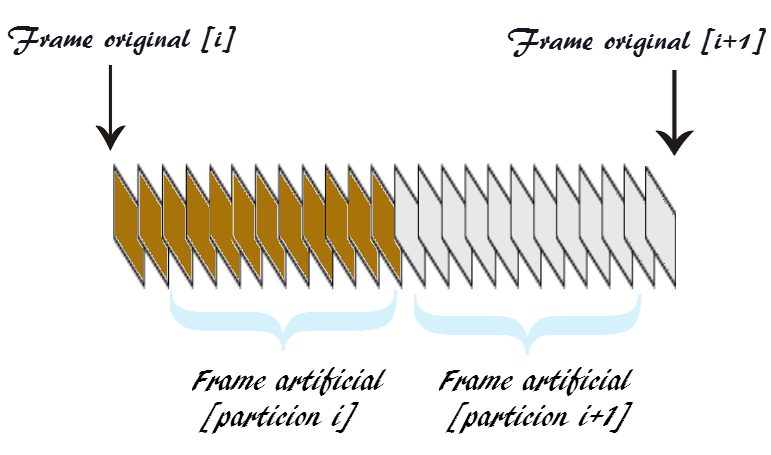
\includegraphics[width=0.55\textwidth]{VecinoCercano.png}
     \caption{Ejemplo de vecino m\'as cercano}
\end{figure}
\noindent

En el caso de la figura, el par\'ametro de cantidad de cuadros a agregar es de $f = 22$. Por ende, se lo divide en dos particiones de $11$ frames artificiales cuya im\'agen corresponder\'a al frame original m\'as cercano (el marr\'on o blanco). Como observaci\'on trivial, el frame original $i$ se lo considera como la im\'agen reproducida en el estado de tiempo anterior a los artificiales agregados de por medio. An\'alogamente, ocurre con el otro cuadro en el extremo derecho.

Volviendo al an\'alisis del video en su mera totalidad, se repite el anterior procedimiento en cada par de frames en el orden concebido por la secuencia del video. De tal forma, se obtienen los frames artificiales, consiguiendo una nueva filmaci\'on con el efecto de $slowmotion$ que este m\'etodo propone. 

\textbf{¿Qu\'e relaci\'on lleva este m\'etodo con el concepto de interpolar?} No dejaremos esta pregunta de lado, pues estar\'iamos ignorando lo que en la introducci\'on le dimos tanta importancia. Como pequeño recordatorio, en interpolaci\'on se buscamos obtener nuevos puntos del plano en base a los datos ya conocidos. Copiar la im\'agen del extremo m\'as cercano equivale a tomar cada p\'ixel del frame original, o sea los datos conocidos, e insertar estos valores en el frame artificial. De hecho, el frame artificial no es m\'as que un ``punto intermedio'' entre los dos frames originales.

Transladamos esto \'ultimo a t\'erminos matem\'aticos para evitar cualquier ambigüedad al respecto. Por cada p\'ixel, se tiene un polinomio al que denominaremos $S_{i,j}$ cuyo \'indice denota a la posici\'on de la matriz del frame que se esta evaluando. Por otro lado, abreviaremos a $frameOriginal_{p}$ al cuadro que esta en el extremo inferior (hecho pasado) y $frameOriginal_{(p+1)}$ al del extremo superior (hecho futuro). Finalmente, $f$ que simboliza nuevamente la cantidad de frames a adicionar. Definimos a $S_{i,j}$ como:

\[
S_{i,j}(x) = 
\left\{
    \begin{array}{ll}
        pixel(frameOriginal_{p}(i,j)) & \mbox{si } x \leq f/2 \\
        \hspace{0.3cm}     
        pixel(frameOriginal_{(p+1)}(i,j)) & \mbox{si } x > f/2
    \end{array}
\right.
\]

(Continuara)

\subsubsection{Construcci\'on mediante Interpolaci\'on lineal}

Semejante al \textit{cuadro m\'as cercano}, en el sentido que comparten la ideolog\'ia de trabajar c\'iclicamente con cada par de frames para eventualmente, obtener el video deseado con su respectivo efecto. No obstante, contaremos lo particular y caracter\'istico de este m\'etodo, que puede propocionar ciertas mejoras en el movimiento de objetos durante su filmaci\'on.

Por un lado, no posee la misma intuici\'on que su antecesora, donde la im\'agen de cada frame artificial se basa en copiar alguno de los dos cuadros originales en evaluaci\'on. En cambio, se busca utilizar fundamentos matem\'aticos que ayuden a \textit{predecir y reflejar} lo sucedido entre cada par de frames del video original. 

Nuevamente, nos enfocamos en analizar el algoritmo propuesto para la creaci\'on de los $n$ frames artificiales que se desean adherir entre cada conjunto de pares. En primer lugar, debemos pensar a cada frame como una matriz de $m$ $x$ $n$ p\'ixeles (dependiendo la resoluci\'on en que se dispone el video), siendo $m$ el largo del cuadro y $n$ el ancho. En segundo lugar, el procedimiento destina a generar un polinomio de grado uno \footnote{ Tambi\'en definida como funci\'on lineal; \url{https://es.wikipedia.org/wiki/Lineal}.} entre ese par de frames originales. Aunque, ¿de qu\'e forma inventaremos dichos polinomios? Para ello, introducimos algunos conceptos que resolver\'an esta inc\'ognita.

Dicho esto, el m\'etodo se centra en crear un polinomio interpolador por cada posici\'on del frame cuyos puntos interpolados \textbf{(creo que no es puntos interpolados, pero no se me ocurre el verdadero)} resultan ser los valores de dicha ubicaci\'on en el par de frames originales que se est\'a trabajando. Por ende, tendremos por cada par de cuadros reales, $m$ $x$ $n$ polinomios de grado uno. De lo anterior, nace una nueva duda : ¿C\'omo esto resuelve nuestro problema de crear m\'utiples frames artificiales?

El hecho esta en que ahora conocemos los valores intermedios entre los dos cuadros originales y en consecuencia, podemos particionar ese dominio en $p$ partes ($p$ siendo la cantidad de frames que se adiciona en cada par) y finalmente, evaluar el polinomio en dicho borde de cada fragmento. Como observaci\'on, este paso lo tendremos que aplicar para cada posici\'on de la im\'agen.

De misma forma, se realiza la tarea sobre cada par agrupado en el orden indicado con lo que eventualmente, el m\'etodo en cuesti\'on concluye con su labor, dejando el efecto de $slowmotion$ que la misma ofrece.

( Cosas para agregar : imagenes o ejemplo sencillo. No se si explicar polinomio interpolado aca o en el desarrollo. Etc. Rta de L: va antes, lo pongo en una sección anterior. Va a haber que reorganizar un poco esto porque nos estamos repitiendo.) 